\documentclass[12 pt, leqno]{article}
\usepackage{latexsym}
\usepackage{amsmath}
\usepackage{amsfonts}
\usepackage{fancyhdr}
\usepackage{graphicx}
\usepackage[margin=1in]{geometry}
\setlength\parindent{20pt}
\usepackage{setspace} 
\newcommand{\indep}{\rotatebox[origin=c]{90}{$\models$}}


\begin{document}

\title{Fixed Effects Summary}
\author{Siddhartha Basu}
\date{\today}
\maketitle


\section{Synopsis of Florencia Class Notes}

\subsection{Introduction}
Panel data contains repeated observations on the same units over time. This allows for a new dimension of richness in our analysis, since we can look at variation within individuals as well as across individuals. 

\textbf{Example:} want to identify the causal effect of marriage on wages. If you just regressed wage on married, you will have endogeneity (taller men get married, taller men have higher wages, etc.) Using panel data, you can exploit over time variation within individuals and use each individual as his or her own control. This helps you get around unobserved selectivity of married men.

$$ Wage_{it} = \beta_0 + \beta_1 M_{it} + \beta_2 X_{it} + \alpha_i + \epsilon_{it}$$

Here, $\alpha_i$ captures unobserved individual level attributes that don't change over time. 

We can think of a composite error term including time-varying and non time-varying components ($\theta_{it} = \alpha_i + \epsilon_{it}$). If we leave $\alpha_i$ in the error term, $M_i$ will be correlated with the composite error term through its correlation with $\alpha_i$.

We can estimate fixed effects with a \textbf{Deviation from Means} estimator:

$$Wage_{it} - \bar{Wage_{it}} = \beta_1 (M_{it} - \bar{M_{it}}) + \beta_2 (X_{it} - \bar{X_{it}}) + (\epsilon_{it} - \bar{\epsilon_{it}})$$

Note that subtracting the means out eliminates the $\alpha_i$. Note that this may assume that marriage is an absorbing state (?). The deviations from means estimator comes from subtracting the \textbf{between subject} model from the full fixed effects model. The between subject model just has one observation per subject, and is of the form:

$$\bar{Wage_i} = \beta_0 + \beta_1 \bar{M_i} + \beta_2 \bar{X_i} + \alpha_i + \bar{\epsilon_{it}}$$

We can also estimate fixed effects using a \textbf{Least Square Dummy Variable} estimator. Here, instead of `subtracting out' $\alpha_i$, you treat it as a dummy variable, and a parameter to be estimated. Adding these dummies gives us an \textbf{individual specific intercept}. LSDV uses only within-individual variation to identify the effect of interest.

\textbf{Limitations of fixed effects} They only account for individual-level time invariant sources of unobserved heterogeneity. The effect of time-invariant covariates (eg. gender, race) cannot be estimated as they are collinear with the $\alpha_i$. 

\textbf{Graphical Intuition} Fixed effects allows for each individual to have their own intercept. This allows to correct for the bias in OLS which is caused by the association between individual intercepts and X values (marriage). 

The graph below, and our specification assumes that the slopes are the same between individuals. This assumption can be relaxed.

\begin{center}
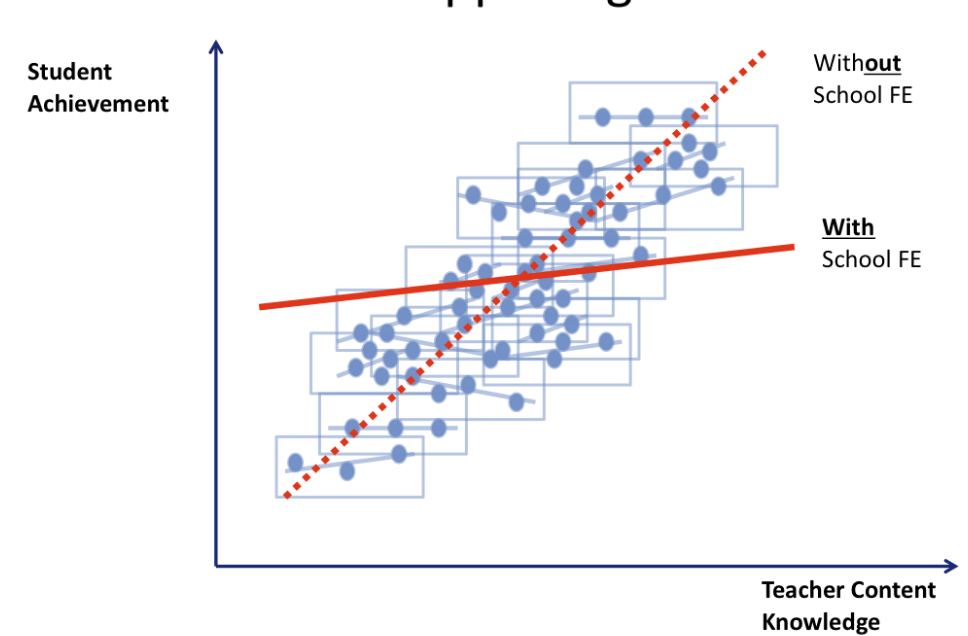
\includegraphics[width = \textwidth]{fixed_effects}
\end{center}

\subsection{Assumptions}

The main assumptions of the fixed effects model are:
\begin{itemize}
\item \textbf{Conditional ignorability"} Treatment is as good as randomly assigned conditional on unobserved time-invariant individual characteristics. In math: $Y(0), Y(1)$ are independent of $M$ conditioned on individual characteristics. 
\item \textbf{Strict exogeneity:} $Cov(x_{it},e_{is}) = 0$ for all $s,t$. Within-individual differences in unobservables $e_{it}$ are independent from within-individual differences in treatment.
\item \textbf{No time-varying confounders:} A confounder in this case 
\begin{itemize}
\item Varies over time.
\item Affects outcome (failing a grade in school)
\item Correlated with treatment (homocides in district)
\item Example: decreasing local law enforcement leads to more homocides, it also leads to worse teacher retention, which leads to lower test scores.
\item A mediator would be more homocides leading to worse teacher retention leading to lower test scores.
\end{itemize}
\item  Effect of treatment on outcome is additive and linear. 
\end{itemize}

Fixed effects do not assume zero correlation between time varying predictor and the observed individual effect:
$$Cov(X_{it}, \alpha_i) = 0 \text{     } \forall t$$
In case this assumption is met, you should use \textbf{random effects}. However most of the time fixed effects are better, since the above assumption is quite hard to meet.

The fixed-effects estimator is very general, and applies to any setting where observations can be grouped together. Consistency just requires a large number of groups.

\subsection{A little bit more on confounders:}

Let $T_{i\cdot}$ be the causal variable of interest, where $i$ is the individual, and $\cdot$ is the index within the individual (e.g. $t$ in the $M_{it}$ context). Then a confound in the fixed effects model:

\begin{itemize}
\item Affects $T_{i\cdot}$ differently across the $\cdot$ variable.
\item Affects y
\end{itemize}

This is often called a `time varying confounder'. \textbf{Strict Exogeneity} requires that $Cov(T_{it}, e_{is}) = 0$ for all s, t (within the individual). Some examples of confounds are:

\begin{itemize}
\item In the twin births example, if we omit gender then, $gender_j$ affects $birthweight_{ij}$ and $testscore_j$. Then $Cov(BW_{ij}, e_{ij}) \neq 0$.
\item In the marriage example, if we omit age, then $age_t$ affects $M_{it}$ as well as $Wage_{it}$, so again $Cov(M_{it}, e_{it}) \neq 0 $
\end{itemize} 

Therefore within-individual varying confounders are one way you can violate strict exogeneity.

One last hypothesis by me. Year fixed effects can get rid of global confounds (e.g. a recession, but not a local one).

\subsection{Details (May 24 lecture)} 

\subsubsection{Standard errors} SE's are bigger when you have fixed effects. Fixed effects exploit only within-individual variation. However, predictors of interest are usually persistent within individual, so only a small portion of the variance is actually used. \textit{You only use a small amount of total variation}

\subsubsection{Fraction of variance that is `between'}

$$\rho = \frac{\sigma_u^2}{\sigma_u^2 + \sigma_e^2}$$

Here $\sigma_u^2$ is the standard deviation between individuals and $\sigma_e^2$ is the standard deviation in $Y$ after we have controlled for the predictor (eg. marital status).

\subsubsection{Intercept in a FE model:} We can write the FE model to be:

$$Wage_{it} = (\beta_0 + \alpha_i) + \beta_1 M_{it} + X'_{it} \beta_2 + \epsilon_{it} $$

We need further constraints on $\beta_0$ and $\alpha_i$ so that we can get unique solutions for them. Examples of constraints are $\beta_0 = 0$ and $\sum{\alpha_i} = 0$. 

\subsubsection{Change in effect of time-invariant predictor over time} While you can't estimate the direct coefficient of gender etc. in a fixed effects model, you can do the following. You can interact these with time dummies to get the change in effect over time. In this case, heterogeneity over time is an issue, as it can lead to confounds. For example, a recession can lead to lower wages and fewer marriages.

\subsubsection{Difference between two years:} Say you want to compute the difference in wages in your data from 1973 and 1977. Then if you have year fixed effects you can do the following t-test:

$$ \frac{b_{77} - b_{73}}{\sqrt{se_{77}^2 + se_{73}^2}} $$

Note that this seems to only work when the $b$ in question is a fixed effect or dummy variable. The general equation for the t-test with a linear restriction $c$ is $\frac{b' c}{s \sqrt{c' (Z'Z)^{-1} c}}$

\subsubsection{Two way fixed effects}

Usually you have to account for heterogeneity associated with both dimensions of panel data: Between individuals (constant over time) and over time (constant across individuals). Easy implementation is adding a set of dummies to capture heterogeneity in the dimension with fewer observations.

\subsubsection{Nonlinear models}

Doing fixed effects with logit is tougher since having perfect prediction (eg. an individual with unchanging dependent variable) prevents estimation in logit. More issues discussed in slides.

\subsubsection{Time distributed fixed effects}

Fixed effects models can be made more flexible to describe the temporal structure of change in $Y$ relative to $t$ through time distributed fixed effects. Eg. in the marriage example:

$$Wage_{it} = \beta_0 + \sum_{p = -s}^{s}{\lambda_p M_{it}^p}  + \beta_2 X_{it} + \alpha_i + \epsilon_{it}$$
 
Where p is the number of years since marriage. For example, you can let control be 2+ years pre-policy implementation, and use 1 year prior to get an anticipation effect. Note that the number of observations in the extreme time points may be low, so standard errors can be large there. 

\subsection{Details (May 31 lecture)} 

\subsubsection{Clustering in Panel Data}

Unit-year observations are assumed to be independent, but in reality, observations of the same unit, or observations for the same year are not independent. This is why you cluster standard errors. Clustered standard errors are generally bigger than non-clustered standard errors.

Serial correlation is another problem. This emerges when current observations of the error term are a function of prior observations (e.g. a societal shock takes more than one period to go away)

\subsubsection{Fixed effects and first differences}

Another way to get rid of the individual specific $\alpha_i$ is by first differencing:

\begin{align*}
Wage_{it} &= \beta_0 + \beta_1 M_{it} + \beta_2 X_{it} + \alpha_i + \epsilon_{it} \\
Wage_{it-1} &= \beta_0 + \beta_1 M_{it-1} + \beta_2 X_{it-1} + \alpha_i + \epsilon_{it-1} \\
\Delta Wage_{it}& = \beta_1 \Delta M_{it} + \beta_2 \Delta X_{it} + \Delta \epsilon_{it}
\end{align*}

Subtracting allows us to drop $\beta_0$ and $\alpha_i$. With two periods, differencing is identical algebraically from deviations from means. This is not the case for 3+ periods. The intuition for this that the fixed effects estimator basically compares $\bar{Y}$ in the years before and after the treatment. First differences estimator looks at $Y$ the year before treatment and the year after. I.e. FD `throws out' data except for right before and right after. 

Both estimators are consistent when all assumptions are met (strict exogeneity). With homoskedastic and serially uncorrelated errors, the deviations from means estimator is more efficient. 

Differences between the two models beyond sampling error suggests either time-varying confounders or time heterogeneity in effects. 

Important: you want to run the regressions for a first difference model without a constant. If you run the model with a constant, the constant ends up becoming the average difference in $Y$ between years, which leads to different results than what we estimated above. Algebraically, let's add in time dummies $\delta_t$:

\begin{align*}
Wage_{it} &= \beta_0 + \beta_1 M_{it} + \beta_2 X_{it} + \delta_t + \alpha_i + \epsilon_{it} \\
Wage_{it-1} &= \beta_0 + \beta_1 M_{it-1} + \beta_2 X_{it-1} + \delta_{t-1}+ \alpha_i + \epsilon_{it-1} \\
\Delta Wage_{it}& = \Delta \delta_t + \beta_1 \Delta M_{it} + \beta_2 \Delta X_{it} + \Delta \epsilon_{it}
\end{align*}

$\Delta \delta_t$ functions as the dummy variable in the above regression.

\subsubsection{Example: effect of birth weight on test scores}

Birthweight is likely correlated with unobservables that affect cognitive performance. If we have data on twins, we can exploit differences in twins' birthweight and differences in test scores to identify the effect of birthweight:

$$Tscore_{ji} = \beta_0 + \beta_1 BW_{ji} + \beta_2 X_{ji} + \alpha_j + e_{ji}$$

Here $j$ indexes the birth, and $i$ indexes the twin. $Tscore$ is test score, $BW$ is birthweight and $X_ji$ is a vector of observed covariates of birthweight that vary across birth (e.g. sex). $\alpha_j$ captures unobserved characteristics of both the mother and the birth. 

\textbf{Key assumption} in this case means that there is no difference between twin A and B that you do not observe that are correlated with both birthweight and $e_{ji}$.

\textbf{Example confound} suppose we don't observe sex. Then sex would be correlated with both birthweight and test scores. 

\subsubsection{Fixed effects vs Random effects: Hausman test}

\textbf{Main random effects assumption:} unit-specific effect $\alpha_i$ is uncorrelated with the causal factor of interest $Cov(X_{it}, \alpha_i) = 0$ for all t. A confound in the case of random effects is an unobserved attribute that is correlated with $X_{it}$ (e.g. marriage) and $Y_i$ (e.g. income). For example, height could be such a confound. 

Random effects allows including time-varying covariates. If zero covariance between individual-specific effect and time varying predictors is met then RE is more efficient than FE. If assumption is not met, then RE is biased!

In reality, the zero-covariance assumption is unlikely to be met. You can use a \textbf{Hausman Test} to understand this in more detail. The null hypothesis will be that $cov(\alpha_i, X_{it}) = 0$. Under $H_0$, $\hat{\beta}_{FE}$ and $\hat{\beta}_{RE}$ are consistent, and $se(\hat{\beta}_{FE}) > se(\hat{\beta}_{RE})$. Under $H_A$, $\hat{\beta}_{RE}$ is inconsistent. The test statistic is:

$$W = \frac{(\hat{\beta}_{FE} - \hat{\beta}_{RE})^2}{Var(\hat{\beta}_{FE}) - Var(\hat{\beta}_{RE})} \sim \chi_1^2$$

\subsubsection{Dynamic panel data models}

DPD models contain one or more lagged dependent variables, which allows for us to model a partial adjustment mechanism. 

$$ Wage_{it} = \beta_0 + \beta_1 M_{it} + \beta_2 X_{it} + Wage_{it-1} + \epsilon_{it}$$

Implicit assumption here is that endogeneity emerges from time-varying pretreatment trends rather than from the time-invariant unit-specific effect.

Combining FE and LDV leads to bias since demeaning/differencing creates a correlation between the lagged DV and error term (Nickell bias, Nickell 1981).

Holtz-Eakin, Newey and Rosen (1988) and Arrellano and Bond (1991) propose a solution where you take first differences to remove the individual effect and then use further lagged terms (in levels and differences) to instrument for the lagged DV in a GMM context. 


\end{document}